\documentclass[aspectratio=169, 12pt]{beamer}
\usepackage{translator}
\usepackage{physics}
\usepackage{graphicx}
\usepackage{siunitx}
\usepackage{amsmath}    % align, align*, \tfrac, \text, etc.
\usepackage{amssymb}    % \mathbb, \mathfrak, extra symbols
\usepackage{amsfonts}   % \mathbb, \mathfrak, \mathcal (loaded by amssymb usually)
\usepackage{mathrsfs}   % \mathscr  <-- the one you asked about
\usepackage{bm}         % \bm{} for bold math
\definecolor{darkred}{RGB}{120,0,0}
\setbeamercolor{structure}{fg=darkred}
\setbeamercolor{title}{fg=darkred}
\setbeamercolor{frametitle}{fg=darkred}
\title{
    Long-term 3+1 simulations of primordial black hole formation during
    radiation domination
}
\subtitle{
	\vspace{1em}
    Submitted: August 13, 2026
}
\author{
    Ning, Z., Cai, R., Wang, S., and Yoo, C.
}
\institute{
    Presented by: Vercil Juan\\
    September 21, 2026
}
\date{}

\begin{document}

\frame{\titlepage}

\begin{frame}{Outline}
	\begin{columns}[T]
		\begin{column}{0.6\textwidth}
			We will discuss the following:
			\begin{itemize}
				\item Preliminaries
				\item Primordial Black Holes
				\item Formulation and Numerical Setup
				\item Numerical Results
				\item Paper Conclusion
			\end{itemize}
		\end{column}
		\begin{column}{0.4\textwidth}
			\centering
			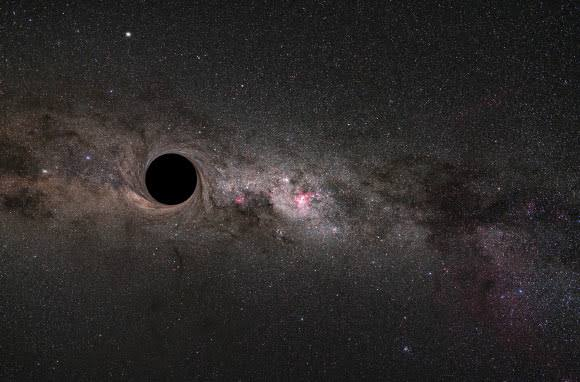
\includegraphics[width=\linewidth, 
			trim = {0 0 6cm 0}, clip
			]{pbh.jpg}
		\end{column}
	\end{columns}
\end{frame}

\begin{frame}{Preliminaries}
	\begin{center}
		{\Large
		Radiation Domination Epoch 
		}	    
	\end{center}

	\begin{figure}[h]
		\centering
		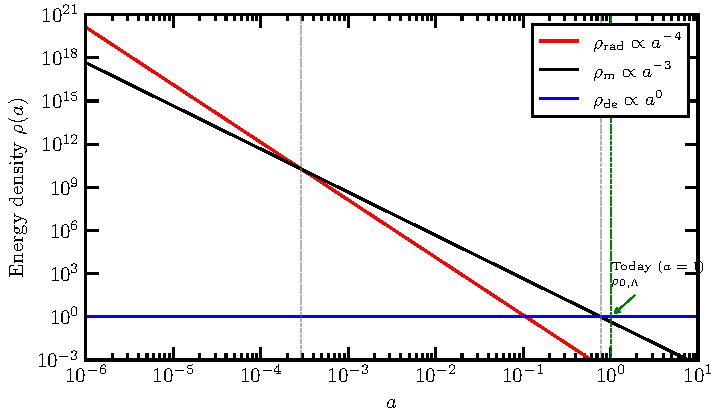
\includegraphics[width=0.7\textwidth]{energy_domination.pdf}
		\caption{Energy density as a function of cosmic scale parameter $a(t)$}
		\label{fig:radiaton-domination}
	\end{figure}
\end{frame}

\begin{frame}{Preliminaries}
	\begin{center}
		{\Large
			Hubble Scale
			\vspace{1em}
		}	    
	\end{center}
	\begin{itemize}
		\item Hubble Parameter $\displaystyle H = \frac{\dot{a}}{a} \sim \SI{70}{km\per\s\per Mpc}$.
			  
			  The hubble parameter, and hence all the following, are functions of time; $H(t)$
		\item Hubble Time $t_H = H^{-1} \approx 14 Gy$
		\item Hubble Radius/Horizon $\displaystyle r_H = \frac{c}{H} \approx$ 4300 Mpc (14 Gly) today
		\item Hubble Mass $\displaystyle M_H = \frac{4\pi}{3}\rho R_H^3 = \frac{c^3}{2GH}
			  \approx \SI{e53}{kg} \sim 10^{23} M_\odot$
	\end{itemize}
\end{frame}

\begin{frame}{Primordial Black Holes}
	\begin{columns}[T]
		\begin{column}{0.6\textwidth}
			\begin{itemize}
				\item Black holes hypothesized to form in the early Universe.
				\item Formed from the direct gravitational collapse of dense matter and radiation
					in the first fractions of a second after the big-bang, rather than
					the late-time collapse of stars.
				\item Can form from sufficiently large primordial curvature perturbations.
				\item The paper studies PBH formation during radiation domination.
			\end{itemize}
		\end{column}
		\begin{column}{0.4\textwidth}
			\centering
			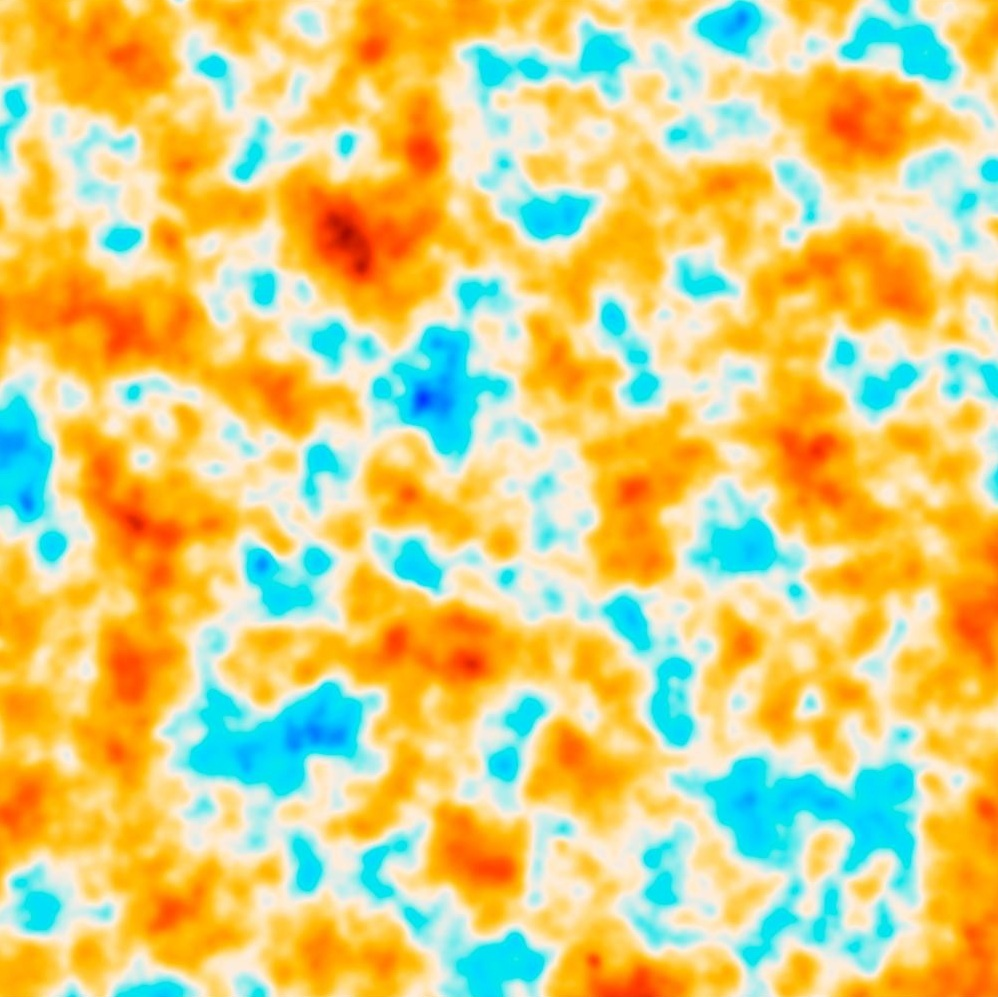
\includegraphics[width=\linewidth, 
			]{cmb.jpg}
		\end{column}
	\end{columns}
\end{frame}
\begin{frame}{Primordial Black Holes}
	\begin{columns}[T]
		\begin{column}{0.5\textwidth}
			Can possibly explain/add information to
			\begin{itemize}
				\item Dark matter
				\item Early gravitational waves
				\item Seeds of supermassive blackholes
				\item Probe early universe physics
			\end{itemize}
		\end{column}
		\pause
		\begin{column}{0.5\textwidth}
			What the paper aims to do
			\begin{itemize}
			    \item Perform a fully $3+1$ dimension numerical relativity simulation of 
					PBH formation
				\item Starting with formation, accretion, and following through 
					its evolution over a long time (order of several Hubble times)
				\item Determine the critical formation parameters, including the
					threshold perturbation amplitude $\mu_c$ and the critical exponent
					$\gamma$ governing the PBH mass scaling.
			\end{itemize}
		\end{column}
	\end{columns}
\end{frame}

\begin{frame}{Primordial Black Holes}
	{\large\bfseries Basic Picture of PBH Formation}
	\begin{columns}[T]
		\begin{column}{0.5\textwidth}
			{
				\small
			\begin{itemize}
				\item After inflation, the Universe is radiation-dominated, and
					  superhorizon curvature perturbations $\zeta(\mathbf{x})$
					  are frozen into the initial conditions.
				\item While a mode is superhorizon ($\lambda > c/H$), causality
					  prevents it from evolving — its amplitude stays fixed.
				\item As the Universe expands, the comoving Hubble radius
					  $c/(aH)$ grows. Once $\lambda = c/H$, the mode
					  \emph{re-enters the horizon} and starts to evolve
					  dynamically.
			\end{itemize}
			}
		\end{column}
		\pause
		\begin{column}{0.5\textwidth}
			\begin{itemize}
				\item The overdense region then faces a competition:
					  \begin{itemize}
						  \item pressure gradients push the fluid outward,
						  \item self-gravity pulls it inward.
					  \end{itemize}
				\item If the amplitude $\mu$ is large enough, $\mu > \mu_c$, gravity wins and the
					  region collapses, an \emph{apparent horizon} forms,
					  signalling the birth of a PBH.
				\item Perturbations below the threshold instead disperse, leaving
					  no black hole behind.
			\end{itemize}
		\end{column}
	\end{columns}
\end{frame}
% \begin{frame}{Formulation}
	% \begin{center}
	% {\large\bfseries Spacetime Evolution}
	% \end{center}
	
	% \begin{itemize}
		% \item Adaptive Mesh Refinement (AMR) handles the \emph{spatial} cost; the \emph{temporal}
		      % cost remains.
		% \item Physical coordinate speeds redshift as $a^{-1}$, so
		      % $\Delta t \propto a\,\Delta x$ should be allowed — but
		      % the standard Gamma-driver blocks it.
		% \item \texttt{GRChombo} + a scaled Gamma-driver
		      % ($b \propto a^{-2}$, $\eta_{\rm GD} \propto a^{-1}$)
		      % permits $\Delta t \propto a\,\Delta x$.
		% \item A conformal-time gauge provides an independent check.
	% \end{itemize}
% \end{frame}

\begin{frame}{Formulation}
	\begin{center}
	{\large\bfseries Spacetime Evolution}
	\end{center}
	
	Write the spacetime metric in the standard $3+1$ form
	\begin{equation}
		\label{eq:metric}
		ds^2 = - a^2 \dd{t}^2 
		+ \gamma_{ij} ( \dd{x}^i + \beta^i )
		(\dd{x}^j + \beta^{j} t)
	\end{equation}
	where $a,\beta^i$, and $\gamma_{ij}$ denote the lapse function,
	shift vector, and spatial metric, respectively. 

	The future-directed unit vector normal to a constant-$t$ hypersurface
	is 
	\[
		n_\mu = (-\alpha,0,0,0)
	\]
\end{frame}


\begin{frame}{Formulation}
	\begin{center}
	{\large\bfseries Spacetime Evolution}
	\end{center}
	
	Define the extrinsic curvature as 
	\begin{equation}
		\label{eq:extrinsic-curvature}
		K_{ij} = 
		- \frac{1}{2\alpha}
		(\partial_t \gamma_{ij} - \mathcal{L}_\beta \gamma_{ij})
	\end{equation}

	Evolve the Einstein equations using the Baumgarte-Shapiro-Shibata-Nakamura
	(BSSN) formulation. 
	\begin{itemize}
	    \item a widely used reformulation of Einstein's equations in numerical relativity that enables stable, long-term simulations of black hole and neutron star spacetimes.
	\end{itemize}	

\end{frame}

\begin{frame}{Formulation}
	\begin{center}
	{\large\bfseries Spacetime Evolution}
	\end{center}
	
	The evolved geometric variables are:
	\[
		\chi \equiv \gamma^{-1/3}, \quad
		\tilde{\gamma}_{ij} \equiv \chi \gamma_{ij}, \quad
		K \equiv \gamma^{ij} K_{ij},
	\]
	\[
		\tilde{A}_{ij} \equiv \chi\left(K_{ij} - \tfrac{1}{3}\gamma_{ij}K\right),
		\quad
		\tilde{\Gamma}^i \equiv \tilde{\gamma}^{jk}\tilde{\Gamma}^i_{jk}.
	\]

	The matter source terms entering the equations are given by the Eulerian projections
	\[
		E \equiv n_\mu n_\nu T^{\mu\nu} \qquad S_i \equiv - \gamma_{i\mu} n_\nu  T^{\mu\nu}
	\]
	\[
		S_{ij} = \gamma_{i\mu} \gamma_{j\nu} T^{\mu\nu} \qquad  S = \gamma^{ij} S_{ij}
	\]

	The Hamiltonian and momentum constraints take the form
	\begin{align*}
		\mathscr{H}&\equiv ^{(3)} R + K^2 - K_{ij} K^{ij} - 16\pi E = 0 \\
		\mathscr{M}_i &\equiv D_j K^j - D_i K - 8\pi S_i = 0
	\end{align*}
\end{frame}

\begin{frame}{Formulation}
	For the radiation dominated Universe, they describe the matter sector 
	as a perfect fluid, with the stress energy tensor as
	\begin{equation}
		\label{eq:Tmu}
		T^{\mu\nu} = (\rho + p) u^\mu u^\nu + p g^{\mu\nu}
	\end{equation}

	\begin{itemize}
	    \item $\rho$ is the proper energy density measured in the fluid rest frame
		\item $p$ is the pressure
		\item $u^\mu$ is the fluid four-velocity
	\end{itemize}

	They adopt a linear barotropic equation of state
	\[
		p = \omega \rho
	\]
	and set $\displaystyle \omega = \frac{1}{3}$ thoughout the simulation.
\end{frame}

\begin{frame}{Primordial Curvature Perturbation}
    The paper uses a spherical Gaussian curvature perturbation
	\begin{equation}
		\label{eq:gauss-curve}
        \zeta(r)
        =
        \mu e^{-k^2r^2}W(r).
	\end{equation}
    \begin{itemize}
        \item $\mu$: amplitude of the perturbation.
        \item $k^{-1}$: characteristic length scale.
        \item $W(r)$: smooth cutoff near the numerical boundary.
    \end{itemize}
\end{frame}
\begin{frame}{Primordial Curvature Perturbation}
	\begin{center}
	{\large\bfseries Window function}
	\end{center}
	\[
		W(r) = \begin{cases}
			1, & 0\leq r \leq r_W\\
			1 - \frac{[(L-r_W)^6 - (L-r)^6]^6}{(L-r_W)^36} ,
			   & r_W < r < L\\
			0, & r\geq L
		\end{cases}
	\]
	\begin{itemize}
	    \item $L$ is the half side length of the cubic simulation
		\item $r_W$ is the radius at which the window begins to taper off.
	\end{itemize}
	
\end{frame}

\begin{frame}{Critical Mass Scaling}
    Near the threshold, the PBH mass obeys
    \[
        M_{\rm BH}
        =
        M_H K(\mu-\mu_c)^\gamma.
    \]

    Here
    \begin{itemize}
        \item $M_H$: Hubble mass,
        \item $K$: proportionality constant,
        \item $\mu_c$: critical perturbation amplitude,
        \item $\gamma$: critical exponent.
    \end{itemize}
\end{frame}
\begin{frame}{Simulation}
	\begin{center}
		{\large\bfseries Numerical Structure\par}
	\end{center}
	\vspace{0.5em}
	\begin{itemize}
	    \item The paper implements the numerical scheme in the open-source numerical-relativity
			code \texttt{GRChombo}, which employs the Chombo library for block adaptic mesh refinement (AMR)
		\item Incorportate the flux-conservative fluid scheme described above into the existing BSSN evolution
			infrastructure
		\item Differentiate the BSSN variables using fourth order finite-difference stencils and update
			the fluid conserved variables through numerical fluxes at cell faces
		\item Integrate the coupled system using the method of
			lines and the classical fourth-order Runge–Kutta scheme.
	\end{itemize}
\end{frame}
\begin{frame}{Simulation}
	\begin{center}
		{\large\bfseries Numerical Structure\par}
	\end{center}
	\vspace{0.5em}
	\begin{itemize}
		\item \textbf{Domain:} evolve on the octant
			  $0 \le x, y, z \le L$ with reflection boundaries —
			  equivalent to a periodic box of side $2L$ for the
			  reflection-symmetric configurations considered here,
			  at $\sim\!8\times$ lower cost; validated against a full
			  periodic run at the same resolution.
		\item \textbf{Resolution:} base grid $64^3$ cells on the octant,
			  five AMR levels with refinement ratio 2 giving
			  $\Delta x_{\min} = L/2048$, refined on gradients of
			  $\chi$ and $E$; for the long accretion runs, $L \to 2$
			  and the base grid is doubled so the physical resolution
			  and AMR criteria are unchanged.
	\end{itemize}
\end{frame}
\begin{frame}{Simulation}
	\begin{center}
		{\large\bfseries Setup\par}
	\end{center}
	\vspace{0.5em}
	\begin{itemize}
		\item The simulation begins with a curvature perturbation
		      $\zeta(\mathbf{x})$ placed \emph{well outside} the
		      Hubble horizon.
		\item Enforced by the small parameter
		      \[
		          \epsilon \equiv \frac{k}{a_i H_i} \ll 1,
		      \]
		      i.e.\ physical wavelength $\gg$ Hubble radius.
		\item In this limit, spatial gradients are suppressed by
		      powers of $\epsilon$ — causality freezes the
		      perturbation's evolution.
		\item The initial slice is therefore clean, unambiguous,
		      and physically motivated: this is what inflation
		      produces.
	\end{itemize}
\end{frame}

\begin{frame}{Simulation}
	\vspace{0.5em}
	\begin{itemize}
		\item Because $\epsilon \ll 1$, the geometric variables can be
		      expanded order-by-order in $\epsilon$ (Shibata--Sasaki).
		\item Through $\mathcal{O}(\epsilon^2)$:
		      \[
		          \chi = a_i^{-2} e^{-2\zeta}\left[1
		          + \frac{2f}{3(1+\omega)}\frac{1}{(a_i H_i)^2}\right]
		          + \mathcal{O}(\epsilon^4),
		      \]
		      and similarly for
		      $\tilde{\gamma}_{ij}$, $K$, $\tilde{A}_{ij}$, $\alpha$.
		\item The fluid variables are then recovered by
		      \emph{solving the Hamiltonian and momentum
		      constraints} — not from the truncated expressions.
		\item Result: constraint-satisfying initial data that
		      exactly represents a superhorizon perturbation.
	\end{itemize}
\end{frame}
\begin{frame}{Simulation}
	\vspace{0.5em}
	\begin{itemize}
		\item The perturbation does \emph{not} move — its comoving
		      wavelength $\lambda_{\rm com} = 2\pi/k$ is constant.
		\item What grows is the \emph{comoving Hubble radius}
		      $c/(aH)$, because $a$ grows and $H$ decreases.
		\item Horizon entry occurs when the two meet:
		      \[
		          a(t_H)\, r_m = H^{-1}(t_H),
		      \]
		      defining
		      $t_H = t_i\,(a_i H_i r_m)^{1/(1-\alpha_\omega)}$
		      and $M_H = t_H/(2\alpha_\omega)$.
		\item After $t_H$, the perturbation is causally connected
		      and begins to evolve dynamically.
	\end{itemize}
\end{frame}
\begin{frame}{Simulation}
	\vspace{0.5em}
	\begin{itemize}
		\item Once subhorizon, the overdense region faces two
		      opposing forces:
		      \begin{itemize}
		          \item \textbf{Pressure gradients} push the radiation
		                fluid outward.
		          \item \textbf{Self-gravity} pulls the region inward.
		      \end{itemize}
		\item The outcome depends on the perturbation amplitude
		      $\mu$:
		      \[
		          \begin{cases}
		              \mu < \mu_c: & \text{dispersal, no PBH}, \\[2pt]
		              \mu > \mu_c: & \text{collapse, PBH forms}.
		          \end{cases}
		      \]
		\item The threshold $\mu_c$ depends on the equation of state
		      and the shape of the curvature profile.
		\item Just above threshold, PBH mass obeys a critical
		      scaling law $M_{\rm BH} \propto (\mu - \mu_c)^{\gamma}$.
	\end{itemize}
\end{frame}
\begin{frame}{Simulation}
	\vspace{0.5em}
	\begin{itemize}
		\item When collapse succeeds, an \emph{apparent horizon}
		      forms — the operational signature of PBH birth.
		\item The mass is measured from the horizon area:
		      \[
		          M_{\rm BH} = \sqrt{A_{\rm AH} / 16\pi}.
		      \]
		\item The paper then follows the PBH for \emph{many Hubble
		      times} after formation, tracking its accretion of the
		      surrounding radiation.
		\item The late-time growth is fit to the
		      Zel'dovich--Novikov law:
		      \[
		          \dot{M}_{\rm BH} = \frac{3F}{2}\frac{M_{\rm BH}^2}{t^2}.
		      \]
		\item This is the ``long-term'' part of the title: the
		      simulation spans horizon entry, collapse, and
		      post-formation accretion.
	\end{itemize}
\end{frame}
\begin{frame}{Cosmological Gauge}
	\begin{itemize}
		\item Standard $1+\log$ slicing drives $\alpha$ away from
		      unity on an expanding background ($K = -3H < 0$).
		      Fix: background-subtracted slicing
		      $(\partial_t - \beta^i \partial_i)\alpha
		      = -2\alpha(K - K_b)$, with $K_b = -3H(t)$.
		\item Physical coordinate speeds redshift as $a^{-1}$, so
		      the CFL limit would permit
		      $\Delta t \propto a(t)\,\Delta x$.
		\item But the Gamma-driver's gauge modes do \emph{not}
		      redshift: they see the \emph{conformal} metric
		      $\tilde{\gamma}_{ij} = \delta_{ij}$, so their
		      characteristic speeds $v_L = \sqrt{4b/3}$ stay
		      $O(1)$ in coordinate units.
		\item Result: a fixed time step, and an increasingly
		      conservative CFL number as the Universe expands.
		\item Scale the Gamma-driver coefficients with $a(t)$:
		      \[
		          b(t) = b_0\!\left[\frac{a_i}{a(t)}\right]^2,
		          \qquad
		          \eta_{\rm GD}(t) = \eta_{\rm GD,0}\,\frac{a_i}{a(t)},
		      \]
		      with $b_0 = 3/4$, $\eta_{\rm GD,0} = 1$.
	\end{itemize}
\end{frame}
\begin{frame}{Cosmological Gauge}
	\vspace{0.5em}
	\begin{itemize}
		\item Then the two stability parameters stay constant when
		      $\Delta t \propto a\,\Delta x$:
		      \[
		          C_\beta \propto \frac{\Delta t}{a\,\Delta x}
		          = \text{const}, \qquad
		          C_\eta \propto \frac{\Delta t}{a} = \text{const}.
		      \]
		\item The driver does \emph{not} turn off: proper-distance
		      gauge speed $a\,v_L$ stays constant; only the
		      convergence rate in cosmic time changes.
		\item \textbf{Independent check:} a conformal-time gauge
		      ($\alpha_\eta = a\alpha_t$, $\beta^i_\eta = a\beta^i_t$)
		      where physical speeds are already constant, so the
		      standard driver with $b = 3/4$, $\eta_{\rm GD} = 1$
		      works directly.
		\item \textbf{Payoff:} $\Delta t$ grows to
		      $\Delta t/t_H \simeq 0.52$ (vs.\ standard cap
		      $2.60\times 10^{-3}$) — a $\sim\!200\times$ larger
		      step and a $\sim\!94\times$ reduction in coarse
		      advances, with identical AH masses and constraints.
	\end{itemize}
\end{frame}
\begin{frame}{Results}
	\begin{center}
    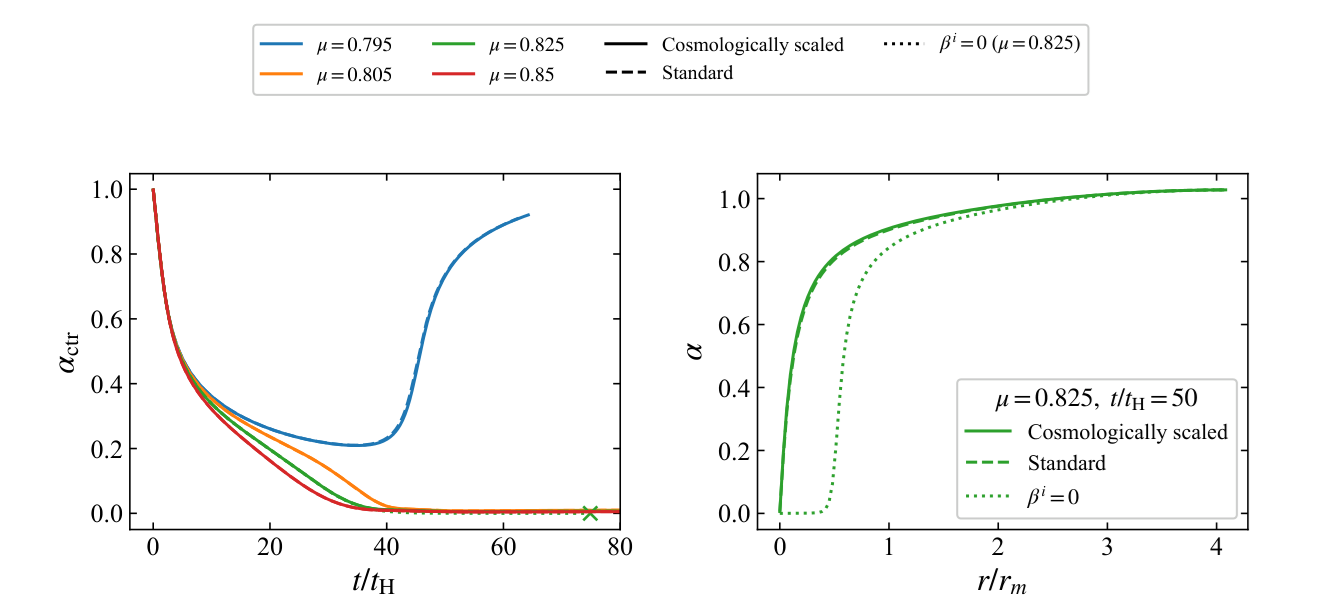
\includegraphics[width=0.9\textwidth]{result1.png}
	\end{center}
\end{frame}
\begin{frame}{Results}
	\begin{center}
    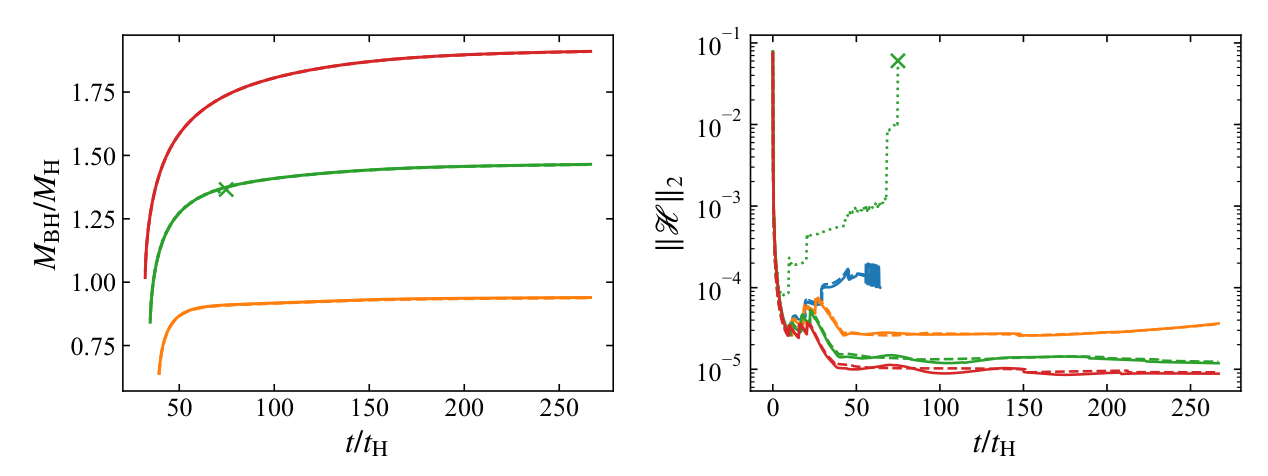
\includegraphics[width=0.9\textwidth]{result2.png}
	\end{center}
\end{frame}
\begin{frame}{Results}
	\begin{center}
    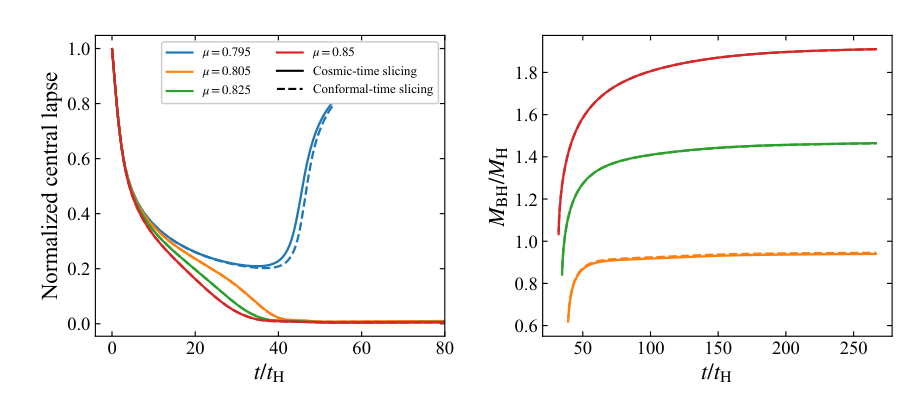
\includegraphics[width=0.9\textwidth]{result3.png}
	\end{center}
\end{frame}
\begin{frame}{Results}
	\begin{center}
    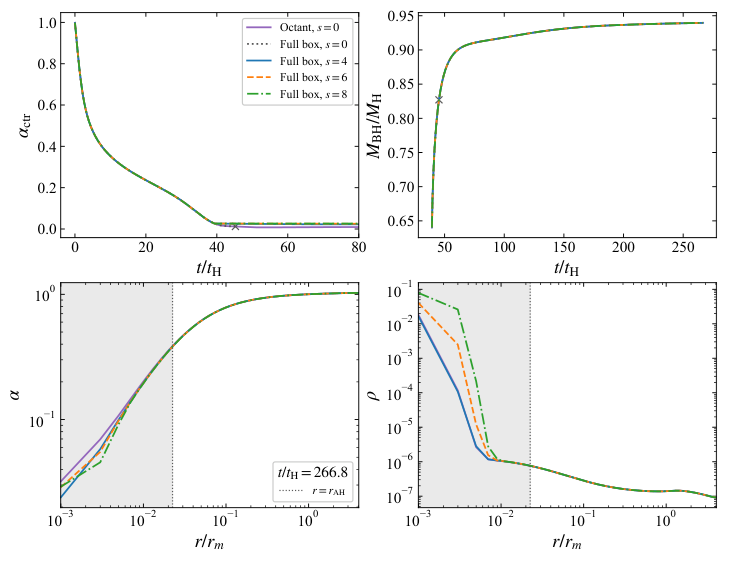
\includegraphics[width=0.7\textwidth]{result4.png}
	\end{center}
\end{frame}
\begin{frame}{Results}
	\begin{center}
    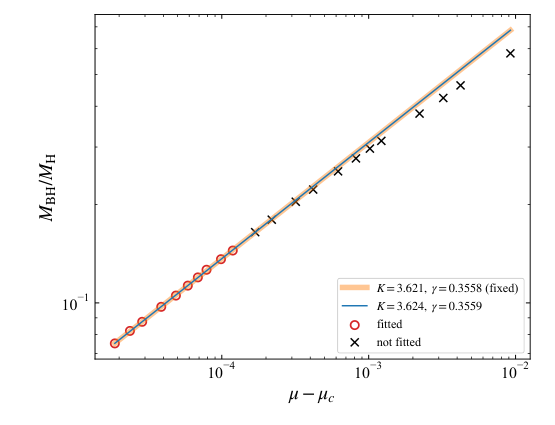
\includegraphics[width=0.7\textwidth]{result5.png}
	\end{center}
\end{frame}

\begin{frame}{Critical Exponent}
    The simulation finds
    \[
        \gamma \simeq 0.3559.
    \]

    Therefore,
    \[
        M_{\rm BH}
        \propto
        (\mu-\mu_c)^{0.3559}.
    \]

    As
    \[
        \mu \rightarrow \mu_c^+,
    \]
    the PBH mass approaches zero in the critical-scaling regime.
\end{frame}

\begin{frame}{Critical Amplitude}
	The simulation finds the collapse threshold
	\[
		\boxed{\,0.79578 < \mu_c < 0.79580\,}
	\]
	refining earlier 3D results and matching the spherically
	symmetric Misner--Sharp value
	$\mu_c \simeq 0.79579 \pm 1\times 10^{-5}$ — a strong
	validation of the 3D fluid evolution.
\end{frame}

\begin{frame}{Conclusion}
	\begin{itemize}
		\item Developed a 3D numerical-relativity framework for PBH formation
		      from superhorizon curvature perturbations during
		      radiation domination.
		\item Cosmologically scaled Gamma-driver gives
		      $\Delta t \propto a\,\Delta x$ — $\sim\!94\times$
		      fewer coarse advances, identical physics.
		\item Threshold $0.79578 < \mu_c < 0.79580$, matching
		      Misner--Sharp; critical exponent
		      $\gamma \simeq 0.3559$, matching the radiation value.
		\item Late-time accretion over many Hubble times fits the Zel'dovich--Novikov law.
		\item First 3D determination of both the critical scaling
		      relation and the post-formation accretion law.
	\end{itemize}
\end{frame}
\begin{frame}[allowframebreaks]{References}
	\begin{thebibliography}{9}
		\setbeamertemplate{bibliography item}[text]   % <-- this line
		\bibitem{ning2026pbh}
		Ning, Z., Cai, R.-G., Wang, S.-J., \& Yoo, C.-M. (2026).
		\textit{Long-term 3+1 simulations of primordial black hole
		formation during radiation domination}.
		arXiv. https://arxiv.org/abs/2608.13206

		\bibitem{carr1975}
		Carr, B. J. (1975).
		The primordial black hole mass spectrum.
		\textit{The Astrophysical Journal}, 201, 1--19.
		https://doi.org/10.1086/153853

		\bibitem{escriva2020}
		Escriva, A. (2020).
		Simulation of primordial black hole formation using
		pseudo-spectral methods.
		\textit{Physics of the Dark Universe}, 27, 100466.
		https://doi.org/10.1016/j.dark.2019.100466
	\end{thebibliography}
\end{frame}
% \begin{frame}{Radiation Domination}
%     During radiation domination,
%     \[
%         a(t)\propto t^{1/2},
%     \]
%     so
%     \[
%         H=\frac{1}{2t}.
%     \]

%     Therefore,
%     \[
%         t_H=H^{-1}=2t
%     \]
%     and
%     \[
%         M_H=\frac{c^3t}{G}.
%     \]
% \end{frame}

% \end{frame}

\end{document}
